\documentclass{article}
\usepackage{geometry}
\usepackage{graphicx}
\geometry{a4paper, margin=1in}
\usepackage{hyperref}

\title{Use Case Specification For Teacher Portal}
\author{}
\date{}

\begin{document}

\maketitle

\section{Introduction}
\subsection{Use-Case Name}
1. Login\\
2. Registration\\
3. Question Bank Management\\
4. Exam Management


\subsection{Brief Description}
The teacher portal is the interface for teachers to manage the question bank and exams. The teacher can log in, register, manage the question bank, and manage exams.
\section{Actors}
The primary actor involved in the use-cases is the \textbf{teacher}.

\section{Use Cases}

\subsection{Login}

\subsubsection{Brief Description}
The teacher logs into the system.
\subsubsection{Use-Case Diagram}
% Insert the login.png image here
\begin{figure}[h]
    \centering
    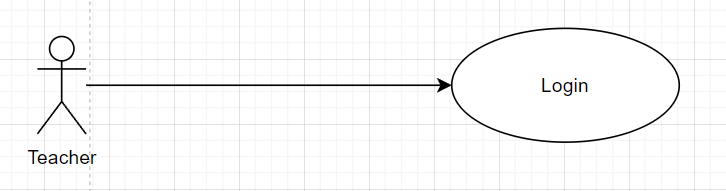
\includegraphics[width=0.5\textwidth]{login.png}
    \caption{Login Use-Case Diagram}
\end{figure}


\subsubsection{Main Flow}
% persudo code
\begin{verbatim}
1. The teacher enters the initial interface of the system.
2. The teacher enters the username and password.
3. The teacher selects the "login" option.
4. The system validates the username and password.
5. The system displays the main interface.
6. The use case ends.
\end{verbatim}

\subsubsection{Alternative Flows}
A1: Incorrect username or password
\begin{verbatim}
At {The system validates the username and password}:
1. If the username or password is incorrect, the system displays an error message.
2. The flow of events is resumed at {The teacher enters the username and password}.
\end{verbatim}


\subsection{Registration}
\subsubsection{Brief Description}
The teacher registers for an account in the system.

\subsubsection{Use-Case Diagram}
% Insert the registration.png image here
\begin{figure}[h]
    \centering
    \includegraphics[width=0.5\textwidth]{registration.png}
    \caption{Registration Use-Case Diagram}
\end{figure}

\subsubsection{Main Flow}
% persudo code
\begin{verbatim}
1. The teacher enters the initial interface of the system.
2. The teacher selects the "register" option.

{Registration}
3. While the teacher in the registration interface:
    3.3.1 The system displays the registration form, including the fields:
        - Username
        - Name
        - Gender 
        - Age
        - Position 
        - Department 
        - Password
        - Password confirmation
    {Filling in the registration form}
    3.3.2 The teacher fills in the registration form.
    {Submitting the registration form}
    3.3.3 The teacher selects the "register" option.
    3.3.4 The system stores the teacher's information and displays a success message.
5. The use case ends 
\end{verbatim}


\subsubsection{Alternative Flows}
A1: Incomplete form
\begin{verbatim}
At {Submitting the registration form}:
1. If the form is incomplete, the system displays an error message.
2. The flow of events is resumed at {Filling in the registration form}.
\end{verbatim}

\noindent A2: Cancel registration
\begin{verbatim}
At any point between {Registration}, 
{Filling in the registration form} and 
{Submitting the registration form}:
1. If the user selects the "close" option.
2. The system returns to the initial interface.
\end{verbatim}

\noindent A3: Username already exists
\begin{verbatim}
At {Submitting the registration form}:
1. The teacher selects the "register" option.
2. If the username already exists, the system displays an error message.
3. The flow of events is resumed at {Filling in the registration form}.
\end{verbatim}

\noindent A4: Passwords do not match
\begin{verbatim}
At {Submitting the registration form}:
1. The teacher selects the "register" option.
2. If the passwords do not match, the system displays an error message.
3. The flow of events is resumed at {Filling in the registration form}.
\end{verbatim}

\subsection{Question Bank Management}

\subsubsection{Beief Description}
The teacher manages the question bank by filtering, adding, updating, and deleting questions.
\subsubsection{Use-Case Diagram}
% Insert the manage_question_bank.png image here
\begin{figure}[h]
    \centering
    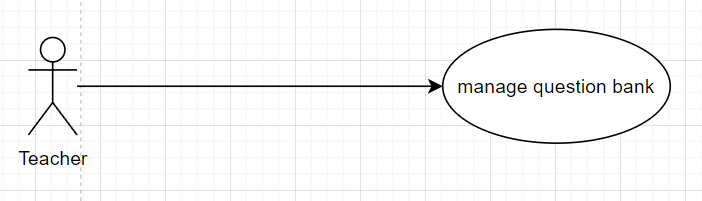
\includegraphics[width=0.5\textwidth]{manage_question_bank.png}
    \caption{Question Bank Management Use-Case Diagram}
\end{figure}

\subsubsection{Main Flow}
% Write the main flow of events in the use-case using persudo code.
\begin{verbatim}
1. User enters the initial interface of the system.
2. User inputs the correct username and password.
3. User selects the "login" option.
4. The system displays the main interface.
5. User selects the "Question Bank" option.
6. The system displays the question bank interface.

{Select Activity}
7. While the teacher in the question bank interface.
    7.1 If the teacher perform FILTERING QUESTIONS
        {Entering filters for questions}
        7.1.1 The teacher fill in/select the filters for the questions,
        including the "Question", "Type", "Score".
        {Filtering questions}
        7.1.2 The teacher clicks the "Filter" button.
        7.1.3 The system displays the list of questions based on the selected filters.
    7.2 If the teacher perform ADDING A NEW QUESTION
        {Entering a new question}
        7.2.1 The teacher enters the "Question", "Type", "Score" and "Answer".
        {Adding a new question}
        7.2.2 The teacher clicks the "Add" button.
        7.2.3 The system stores the information of the new question
         and displays a success message.
    7.3 If the teacher perform UPDATING A QUESTION
        {Updating a question}
        7.3.1 The teacher selects a question from the list of questions.
        7.3.2 The system  highlights the selected question.
        7.3.3 The teacher updates the information of the question.
        7.3.4 The teacher clicks the "Update" button.
        7.3.5 The system updates the information of the question 
        and displays a success message.
    7.4 If the teacher perform DELETING A QUESTION
        {Deleting a question}
        7.4.1 The teacher selects a question from the list of questions.
        7.4.2 The system  highlights the selected question.
        7.4.3 The teacher clicks the "Delete" button.
        7.4.4 The system deletes the question and 
        displays a success message.
8. The use case ends.    
\end{verbatim}
\subsubsection{Alternative Flows}
\noindent A1: Cancel activity
\begin{verbatim}
At any point between {Entering filters for questions},
{Filtering questions}, {Entering a new question},
{Adding a new question}, {Updating a question} and {Deleting a question}:
1. The teacher can cancel the activity.
2. The flow of events is resumed at {Select Activity}.
\end{verbatim}

\noindent A2: Incomplete form of filter questions
\begin{verbatim}
At {Filtering questions}:
1. If the form is incomplete, the system displays an error message.
2. The flow of events is resumed at {Entering filters for questions}.
\end{verbatim}

\noindent A3: Incomplete form of adding a new question
\begin{verbatim}
At {Adding a new question}:
1. If the form is incomplete, the system displays an error message.
2. The flow of events is resumed at {Entering a new question}.
\end{verbatim}

\noindent A4: Incomplete form of updating a question
\begin{verbatim}
At {Updating a question}:
1. If the form is incomplete, the system displays an error message.
2. The flow of events is resumed at {Updating a question}.
\end{verbatim}

\subsection{Exam Management}
\subsubsection{Brief Description}
This use case describes the process of managing exams by the teacher.
\subsubsection{Use-Case Diagram}
% Insert the manage_question_bank.png image here
\begin{figure}[h]
    \centering
    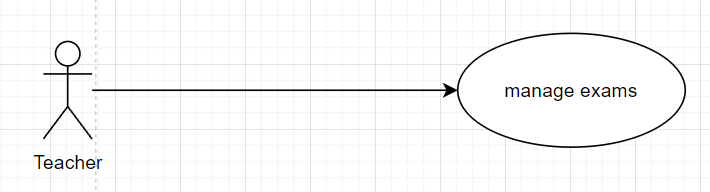
\includegraphics[width=0.5\textwidth]{manage_exams.png}
    \caption{Exam Management Use-Case Diagram}
\end{figure}

% TODO 
\subsubsection{Main Flow}
% Write the main flow of events in the use-case using persudo code.
\begin{verbatim}
1. User enters the initial interface of the system.
2. User inputs the correct username and password.
3. User selects the "login" option.
4. The system displays the main interface.
5. User selects the "Exam" option.
6. The system displays the exam management interface.

{Select Activity}
7. While the teacher has an activity to perform
    7.1 If the teacher perform  FILTER CURRENT EXAM
        {Entering filters for current exams}
        7.1.1 The teacher enters the "Exam Name",
        selects the "CourseID" and select the state of 
        "Published/Unpublished" for filtering the current exam.
        {Filtering current exams}
        7.1.2 The teacher clicks the "Filter" button.
        7.1.3 The system retrieves the list of exams based on the 
        selected filters and display them in the list of current exams.
    7.2 If the teacher perform FILTERING EXISTING QUESTIONS
        {Entering filters for questions}
        7.2.1 The teacher fill in/select the filters for the questions,
        including the "Question", "Type", "Score".
        {Filtering existing questions}
        7.2.2 The teacher clicks the "Filter" button.
        7.2.3 The system displays the list of questions based on the selected filters.
    7.3 If the teacher perform CREATE NEW EXAM 
        {Choosing exam questions}
        7.3.1 The teacher choose the questions from existing questions.
        7.3.2 The system displays the detail of 
        {Entering exam details}
        7.3.2 The teacher enters "New Exam Name", "New Exam Time" 
        and selects the providing courseID and 
        providing option to publish it or not.
        7.3.3 If the teacher press the "Add" button
            {Adding a new exam}
            7.3.3.1 The system adds stores the information 
            of the new exam and displays a success message.
        7.3.4 If the teach press the "Update" button
            {Updating an exam}
            7.3.3.1 The system updates the information of the exam
            and displays a success message.
8. The use case ends.
\end{verbatim}
\subsubsection{Alternative Flows}
\noindent A1: Cancel activity
\begin{verbatim}
At any point between {Entering filters for current exams},
{Filtering current exams}, {Entering filters for questions},
{Filtering existing questions}, {Choosing exam questions},
{Entering exam details}, {Adding a new exam} and {Updating an exam}:
1. The teacher can cancel the activity.
2. The flow of events is resumed at {Select Activity}.
\end{verbatim}

\noindent A2: Incomplete form of filter current exams
\begin{verbatim}
At {Filtering current exams}:
1. If the form is incomplete, the system displays an error message.
2. The system displays the exam management interface.
3. The flow of events is resumed at {Entering filters for current exams}.
\end{verbatim}

\noindent A3: Incomplete form of filter existing questions
\begin{verbatim}
At {Filtering existing questions}:
1. If the form is incomplete, the system displays an error message.
2. The system displays the exam management interface.
3. The flow of events is resumed at {Entering filters for questions}.
\end{verbatim}

\noindent A4: Incomplete form of creating a new exam
\begin{verbatim}
At {Adding a new exam}:
1. If the form is incomplete, the system displays an error message.
2. The system displays the exam management interface.
3. The flow of events is resumed at {Entering exam details}.
\end{verbatim}
\end{document}